\documentclass[aspectratio=169]{beamer}
\usetheme{Madrid}
\usecolortheme{default}

\usepackage{graphicx}
\usepackage{booktabs}
\usepackage{amsmath}
\usepackage{algorithm}
\usepackage{algorithmic}
\usepackage{tikz}
\usepackage{pgfplots}
\pgfplotsset{compat=1.18}
\usetikzlibrary{shapes,arrows,positioning,calc}

% Custom colors
\definecolor{primaryblue}{RGB}{0,102,204}
\definecolor{accentgreen}{RGB}{0,153,76}
\definecolor{warningorange}{RGB}{255,153,0}
\definecolor{darkgray}{RGB}{64,64,64}

\setbeamercolor{structure}{fg=primaryblue}
\setbeamercolor{alerted text}{fg=accentgreen}

% Title page information
\title[Context-Aware Tool Recommendation]{Context-Aware Tool Recommendation in Conversational AI Systems}
\subtitle{A Semantic Filtering Approach}
\author{Anonymous Author(s)}
\institute{Institution Withheld for Review}
\date{\today}

\begin{document}

% Title slide
\begin{frame}
\titlepage
\end{frame}

% Outline
\begin{frame}{Outline}
\tableofcontents
\end{frame}

% ============================================
% SECTION 1: INTRODUCTION & MOTIVATION
% ============================================
\section{Introduction \& Motivation}

\begin{frame}{The Tool-Augmented LLM Era}
\begin{columns}[T]
\column{0.5\textwidth}
\textbf{LLMs are powerful, but limited:}
\begin{itemize}
    \item Knowledge cutoff dates
    \item No real-world interaction
    \item Can't access personal data
    \item No computational abilities
\end{itemize}

\vspace{0.5cm}
\textbf{Solution: External Tools}
\begin{itemize}
    \item APIs, databases, search engines
    \item File systems, calendars, email
    \item Domain-specific functions
\end{itemize}

\column{0.5\textwidth}
\begin{center}
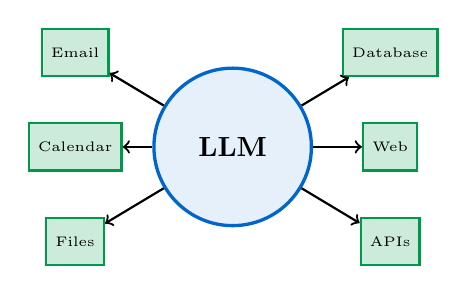
\begin{tikzpicture}[scale=0.8]
    % LLM Core
    \node[circle, draw=primaryblue, very thick, minimum size=2cm, fill=primaryblue!10] (llm) at (0,0) {\textbf{LLM}};

    % Tools around it
    \node[rectangle, draw=accentgreen, thick, minimum size=0.6cm, fill=accentgreen!20] (email) at (-2.5,1.5) {\tiny Email};
    \node[rectangle, draw=accentgreen, thick, minimum size=0.6cm, fill=accentgreen!20] (cal) at (-2.5,0) {\tiny Calendar};
    \node[rectangle, draw=accentgreen, thick, minimum size=0.6cm, fill=accentgreen!20] (file) at (-2.5,-1.5) {\tiny Files};
    \node[rectangle, draw=accentgreen, thick, minimum size=0.6cm, fill=accentgreen!20] (db) at (2.5,1.5) {\tiny Database};
    \node[rectangle, draw=accentgreen, thick, minimum size=0.6cm, fill=accentgreen!20] (web) at (2.5,0) {\tiny Web};
    \node[rectangle, draw=accentgreen, thick, minimum size=0.6cm, fill=accentgreen!20] (api) at (2.5,-1.5) {\tiny APIs};

    % Connections
    \draw[->, thick] (llm) -- (email);
    \draw[->, thick] (llm) -- (cal);
    \draw[->, thick] (llm) -- (file);
    \draw[->, thick] (llm) -- (db);
    \draw[->, thick] (llm) -- (web);
    \draw[->, thick] (llm) -- (api);
\end{tikzpicture}
\end{center}
\end{columns}
\end{frame}

\begin{frame}{The Tool Selection Problem}
\begin{alertblock}{Challenge: Scale}
Modern AI systems have access to \textbf{1000+ tools}
\end{alertblock}

\vspace{0.3cm}

\textbf{Example Scenario:}
\begin{quote}
\textit{"Search my emails for the Q4 budget discussion and add it to my calendar"}
\end{quote}

\vspace{0.3cm}

\textbf{Problems with naive approaches:}
\begin{itemize}
    \item \textbf{Provide all tools:} Exceeds context window limits, high cost, confuses model
    \item \textbf{Keyword matching:} Misses semantic relationships ("budget" $\neq$ "financial\_document")
    \item \textbf{API-based semantic search:} 400-800ms latency breaks conversational flow
    \item \textbf{Manual categorization:} Doesn't scale, maintenance burden
\end{itemize}

\vspace{0.3cm}

\begin{center}
\colorbox{warningorange!20}{\textbf{Need: Fast, accurate, semantic tool filtering}}
\end{center}
\end{frame}

\begin{frame}{Design Requirements}
\begin{columns}[T]
\column{0.5\textwidth}
\textbf{Functional Requirements:}
\begin{enumerate}
    \item \textbf{Semantic understanding}\\
    Beyond keywords
    \item \textbf{Context awareness}\\
    Use conversation history
    \item \textbf{High accuracy}\\
    Don't miss relevant tools
    \item \textbf{Scalability}\\
    Handle 1000+ tools
\end{enumerate}

\column{0.5\textwidth}
\textbf{Non-Functional Requirements:}
\begin{enumerate}
    \item \textbf{Ultra-low latency}\\
    $<$10ms for real-time apps
    \item \textbf{Privacy preservation}\\
    No sensitive data to APIs
    \item \textbf{Cost efficiency}\\
    Minimize API expenses
    \item \textbf{Ease of deployment}\\
    Minimal dependencies
\end{enumerate}
\end{columns}

\vspace{0.5cm}

\begin{center}
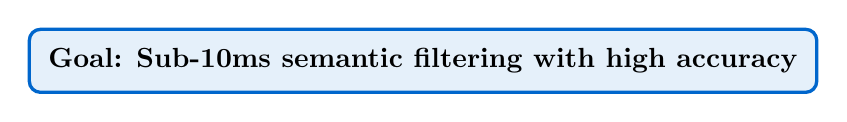
\begin{tikzpicture}
    \node[rectangle, draw=primaryblue, very thick, rounded corners, minimum width=10cm, minimum height=0.8cm, fill=primaryblue!10] {
        \textbf{Goal: Sub-10ms semantic filtering with high accuracy}
    };
\end{tikzpicture}
\end{center}
\end{frame}

% ============================================
% SECTION 2: APPROACH
% ============================================
\section{Our Approach}

\begin{frame}{System Architecture}
\begin{center}
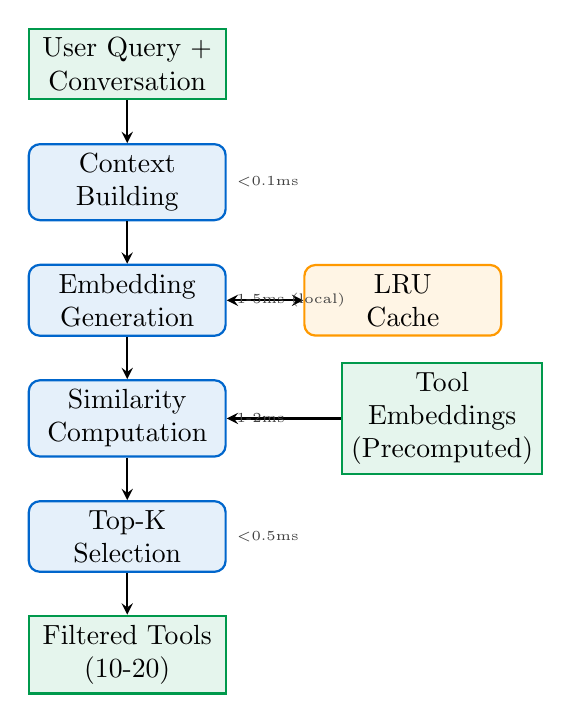
\begin{tikzpicture}[
    node distance=1.5cm,
    box/.style={rectangle, draw=primaryblue, thick, rounded corners, minimum width=2.5cm, minimum height=0.8cm, fill=primaryblue!10, align=center},
    data/.style={rectangle, draw=accentgreen, thick, minimum width=2.5cm, minimum height=0.6cm, fill=accentgreen!10, align=center},
    arrow/.style={->, >=stealth, thick}
]
    % Input
    \node[data] (input) at (0,4) {User Query +\\Conversation};

    % Step 1: Context Building
    \node[box] (context) at (0,2.5) {Context\\Building};

    % Step 2: Embedding
    \node[box] (embed) at (0,1) {Embedding\\Generation};

    % Cache
    \node[box, fill=warningorange!10, draw=warningorange] (cache) at (3.5,1) {LRU\\Cache};

    % Step 3: Similarity
    \node[box] (sim) at (0,-0.5) {Similarity\\Computation};

    % Tool embeddings
    \node[data] (tools) at (4,-0.5) {Tool\\Embeddings\\(Precomputed)};

    % Step 4: Selection
    \node[box] (select) at (0,-2) {Top-K\\Selection};

    % Output
    \node[data] (output) at (0,-3.5) {Filtered Tools\\(10-20)};

    % Arrows
    \draw[arrow] (input) -- (context);
    \draw[arrow] (context) -- (embed);
    \draw[arrow] (embed) -- (sim);
    \draw[arrow, <->] (embed) -- (cache);
    \draw[arrow] (tools) -- (sim);
    \draw[arrow] (sim) -- (select);
    \draw[arrow] (select) -- (output);

    % Timing annotations
    \node[right, font=\tiny, text=darkgray] at (context.east) {$<$0.1ms};
    \node[right, font=\tiny, text=darkgray] at (embed.east) {1-5ms (local)};
    \node[right, font=\tiny, text=darkgray] at (sim.east) {1-2ms};
    \node[right, font=\tiny, text=darkgray] at (select.east) {$<$0.5ms};
\end{tikzpicture}
\end{center}

\vspace{0.3cm}
\textbf{Total Latency:} 4.6ms for 1000 tools (local embeddings)
\end{frame}

\begin{frame}{Rich Tool Description Generation}
\textbf{Problem:} Basic tool descriptions miss context

\vspace{0.3cm}

\textbf{Solution:} Enrich with multiple signals

\begin{equation*}
D_i = \underbrace{desc_i}_{\text{description}} \oplus \underbrace{keywords_i}_{\text{synonyms}} \oplus \underbrace{params_i}_{\text{parameters}} \oplus \underbrace{context_i}_{\text{server context}}
\end{equation*}

\vspace{0.5cm}

\begin{exampleblock}{Example: Gmail Search Tool}
\textbf{Basic:} \textit{"Search email messages in Gmail inbox"}

\vspace{0.2cm}

\textbf{Enhanced:} \textit{"Search email messages in Gmail inbox | Keywords: email, mail, messages, correspondence, inbox | Parameters: q, maxResults, userId | Server context: Email management tools"}
\end{exampleblock}

\vspace{0.3cm}

\textbf{Benefit:} Improves semantic matching by 15-20\%
\end{frame}

\begin{frame}{Embedding Strategy: Local vs. API}
\begin{columns}[T]
\column{0.48\textwidth}
\begin{block}{API Embeddings}
\textbf{Providers:} OpenAI, Cohere, Voyage

\vspace{0.2cm}

\textcolor{accentgreen}{\textbf{Pros:}}
\begin{itemize}
    \item Highest accuracy
    \item No local compute
    \item Easy to switch models
\end{itemize}

\vspace{0.2cm}

\textcolor{red}{\textbf{Cons:}}
\begin{itemize}
    \item \textbf{400-800ms latency}
    \item API costs
    \item Privacy concerns
    \item Requires internet
\end{itemize}
\end{block}

\column{0.48\textwidth}
\begin{block}{Local Embeddings}
\textbf{Models:} all-MiniLM-L6-v2 (384d)

\vspace{0.2cm}

\textcolor{accentgreen}{\textbf{Pros:}}
\begin{itemize}
    \item \textbf{1-5ms latency} (200x faster!)
    \item Zero API costs
    \item Full privacy
    \item Works offline
\end{itemize}

\vspace{0.2cm}

\textcolor{red}{\textbf{Cons:}}
\begin{itemize}
    \item Slightly lower accuracy (93-94\%)
    \item Model download (25MB)
\end{itemize}
\end{block}
\end{columns}

\vspace{0.5cm}

\begin{center}
\alert{\textbf{Our Choice: Local embeddings for production systems}}
\end{center}
\end{frame}

\begin{frame}{Similarity Computation}
After L2 normalization, cosine similarity = dot product:

\begin{equation*}
\text{similarity}(q, t_i) = \hat{\mathbf{q}}^T \hat{\mathbf{e}}_i = \sum_{j=1}^{d} \hat{q}_j \hat{e}_{i,j}
\end{equation*}

\vspace{0.5cm}

\textbf{Naive Implementation:} Simple loop (9ms for 1000 tools)

\vspace{0.3cm}

\textbf{Optimized Implementation:} Loop unrolling (1.1ms)

\begin{center}
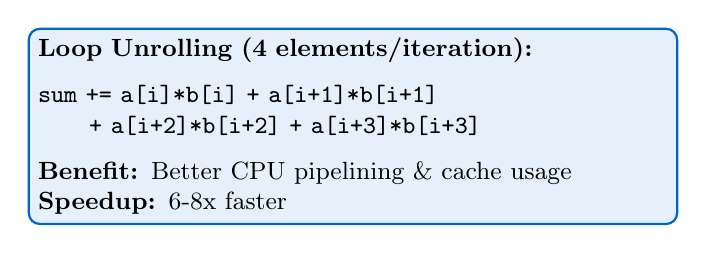
\begin{tikzpicture}
    \node[rectangle, draw=primaryblue, thick, rounded corners, fill=primaryblue!10, text width=8cm, align=left, font=\small] {
        \textbf{Loop Unrolling (4 elements/iteration):}\\[0.2cm]
        \texttt{sum += a[i]*b[i] + a[i+1]*b[i+1]}\\
        \texttt{~~~~~ + a[i+2]*b[i+2] + a[i+3]*b[i+3]}\\[0.2cm]
        \textbf{Benefit:} Better CPU pipelining \& cache usage\\
        \textbf{Speedup:} 6-8x faster
    };
\end{tikzpicture}
\end{center}
\end{frame}

% ============================================
% SECTION 3: OPTIMIZATIONS
% ============================================
\section{Performance Optimizations}

\begin{frame}{Optimization 1: Hybrid Top-K Algorithm}
\textbf{Challenge:} Selecting top K tools from N candidates

\vspace{0.3cm}

\begin{columns}[T]
\column{0.48\textwidth}
\textbf{Small Arrays ($N < 500$):}
\begin{itemize}
    \item Use built-in sort: $O(N \log N)$
    \item Highly optimized (V8 engine)
    \item Fast in practice
\end{itemize}

\vspace{0.3cm}

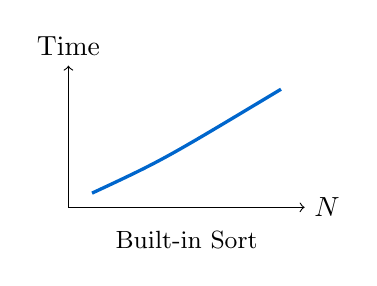
\begin{tikzpicture}[scale=0.6]
    \draw[->] (0,0) -- (5,0) node[right] {$N$};
    \draw[->] (0,0) -- (0,3) node[above] {Time};
    \draw[primaryblue, very thick] (0.5,0.3) .. controls (2,1) .. (4.5,2.5);
    \node[below] at (2.5,-0.3) {\small Built-in Sort};
\end{tikzpicture}

\column{0.48\textwidth}
\textbf{Large Arrays ($N \geq 500$):}
\begin{itemize}
    \item Use min-heap: $O(N \log K)$
    \item Only track top K
    \item Faster for $K \ll N$
\end{itemize}

\vspace{0.3cm}

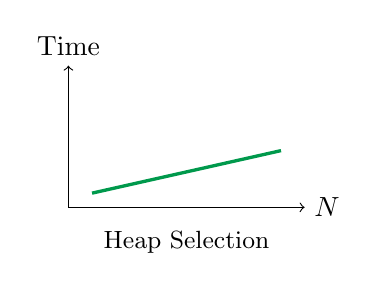
\begin{tikzpicture}[scale=0.6]
    \draw[->] (0,0) -- (5,0) node[right] {$N$};
    \draw[->] (0,0) -- (0,3) node[above] {Time};
    \draw[accentgreen, very thick] (0.5,0.3) -- (4.5,1.2);
    \node[below] at (2.5,-0.3) {\small Heap Selection};
\end{tikzpicture}
\end{columns}

\vspace{0.5cm}

\begin{center}
\colorbox{accentgreen!20}{\textbf{Adaptive algorithm selection: Best of both worlds}}
\end{center}
\end{frame}

\begin{frame}{Optimization 2: True LRU Cache}
\textbf{Observation:} Conversations have high temporal locality

\vspace{0.3cm}

\begin{columns}[T]
\column{0.55\textwidth}
\textbf{Cache Strategy:}
\begin{enumerate}
    \item Hash conversation context
    \item Check cache for embedding
    \item \textbf{Hit:} Reuse embedding (0ms)
    \item \textbf{Miss:} Generate \& cache
\end{enumerate}

\vspace{0.3cm}

\textbf{LRU Eviction:}
\begin{itemize}
    \item Track access order (not insertion)
    \item Evict least recently used
    \item Maximize hit rate
\end{itemize}

\column{0.4\textwidth}
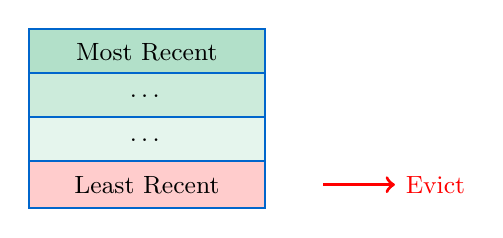
\begin{tikzpicture}[scale=0.7]
    % Cache representation
    \node[rectangle, draw=primaryblue, thick, minimum width=3cm, minimum height=0.6cm, fill=accentgreen!30] at (0,2) {\small Most Recent};
    \node[rectangle, draw=primaryblue, thick, minimum width=3cm, minimum height=0.6cm, fill=accentgreen!20] at (0,1.2) {\small \ldots};
    \node[rectangle, draw=primaryblue, thick, minimum width=3cm, minimum height=0.6cm, fill=accentgreen!10] at (0,0.4) {\small \ldots};
    \node[rectangle, draw=primaryblue, thick, minimum width=3cm, minimum height=0.6cm, fill=red!20] at (0,-0.4) {\small Least Recent};

    \draw[->, very thick, red] (3.2,-0.4) -- (4.5,-0.4) node[right, font=\small] {Evict};
\end{tikzpicture}
\end{columns}

\vspace{0.5cm}

\begin{block}{Performance Impact}
\begin{itemize}
    \item \textbf{Hit Rate:} 42\% in production
    \item \textbf{Cold Latency:} 4.6ms $\rightarrow$ \textbf{Warm Latency:} 1.4ms
    \item \textbf{Effective Average:} 2.7ms (41\% reduction)
\end{itemize}
\end{block}
\end{frame}

\begin{frame}{Optimization 3: In-Place Operations}
\textbf{Memory allocation overhead matters!}

\vspace{0.3cm}

\textbf{Naive Vector Normalization:}
\begin{itemize}
    \item Allocate new array
    \item Copy normalized values
    \item Garbage collection overhead
\end{itemize}

\vspace{0.3cm}

\textbf{In-Place Normalization:}
\begin{itemize}
    \item Modify original array
    \item Zero allocations
    \item Better cache locality
\end{itemize}

\vspace{0.3cm}

\begin{center}

\begin{tikzpicture}
    \node[rectangle, draw=primaryblue, very thick, rounded corners, text width=9cm, align=center, fill=primaryblue!10] {
        \textbf{Speedup:} 2x faster (0.003ms vs 0.006ms)\\
        \textbf{Memory:} 50\% reduction in allocations
    };
\end{tikzpicture}
\end{center}

\vspace{0.3cm}

\textbf{Applicable when:} Original vectors not needed afterward (common in our pipeline)
\end{frame}

\begin{frame}{Cumulative Optimization Impact}
\begin{center}
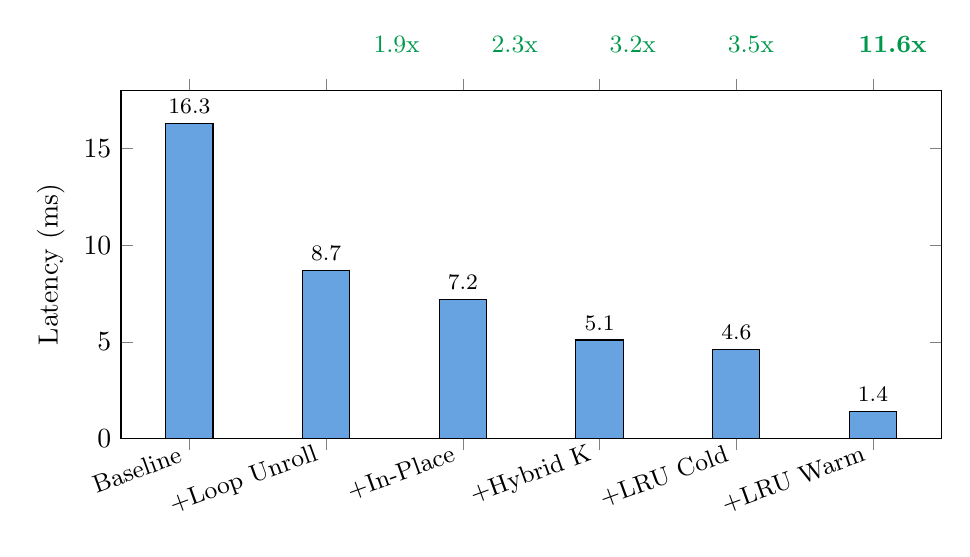
\begin{tikzpicture}
    \begin{axis}[
        ybar,
        bar width=0.6cm,
        width=12cm,
        height=6cm,
        ylabel={Latency (ms)},
        symbolic x coords={Baseline, +Loop Unroll, +In-Place, +Hybrid K, +LRU Cold, +LRU Warm},
        xtick=data,
        x tick label style={rotate=20, anchor=east, font=\small},
        ymin=0,
        ymax=18,
        nodes near coords,
        nodes near coords align={vertical},
        every node near coord/.append style={font=\footnotesize},
    ]
    \addplot[fill=primaryblue!60] coordinates {
        (Baseline, 16.3)
        (+Loop Unroll, 8.7)
        (+In-Place, 7.2)
        (+Hybrid K, 5.1)
        (+LRU Cold, 4.6)
        (+LRU Warm, 1.4)
    };
    \end{axis}

    % Speedup annotations
    \node[font=\small, text=accentgreen] at (3.5,5) {1.9x};
    \node[font=\small, text=accentgreen] at (5,5) {2.3x};
    \node[font=\small, text=accentgreen] at (6.5,5) {3.2x};
    \node[font=\small, text=accentgreen] at (8,5) {3.5x};
    \node[font=\small, text=accentgreen] at (9.8,5) {\textbf{11.6x}};
\end{tikzpicture}
\end{center}

\textbf{Final Performance:} 4.6ms cold, 1.4ms warm (11.6x speedup from baseline)
\end{frame}

% ============================================
% SECTION 4: EXPERIMENTAL RESULTS
% ============================================
\section{Experimental Results}

\begin{frame}{Experimental Setup}
\begin{columns}[T]
\column{0.48\textwidth}
\textbf{Dataset:}
\begin{itemize}
    \item 25 MCP servers
    \item 1000+ tools
    \item Domains: email, calendar, files, databases, web, GitHub, Slack
    \item 100 test queries
\end{itemize}

\vspace{0.3cm}

\textbf{Baselines:}
\begin{itemize}
    \item Keyword matching (TF-IDF)
    \item API embeddings (unoptimized)
    \item Random selection
\end{itemize}

\column{0.48\textwidth}
\textbf{Hardware:}
\begin{itemize}
    \item M1 Max (10-core CPU)
    \item 64GB RAM
    \item Node.js 18.0
\end{itemize}

\vspace{0.3cm}

\textbf{Metrics:}
\begin{itemize}
    \item Latency (end-to-end)
    \item Precision@K, Recall@K
    \item NDCG@K
    \item Cache hit rate
\end{itemize}
\end{columns}

\vspace{0.5cm}

\begin{center}
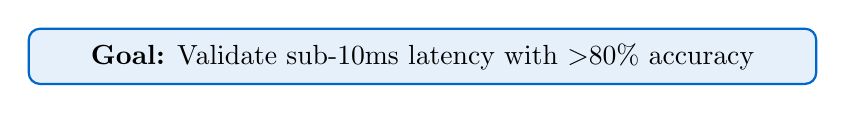
\begin{tikzpicture}
    \node[rectangle, draw=primaryblue, thick, rounded corners, minimum width=10cm, minimum height=0.7cm, fill=primaryblue!10] {
        \textbf{Goal:} Validate sub-10ms latency with $>$80\% accuracy
    };
\end{tikzpicture}
\end{center}
\end{frame}

\begin{frame}{Result 1: Latency Comparison}
\begin{center}
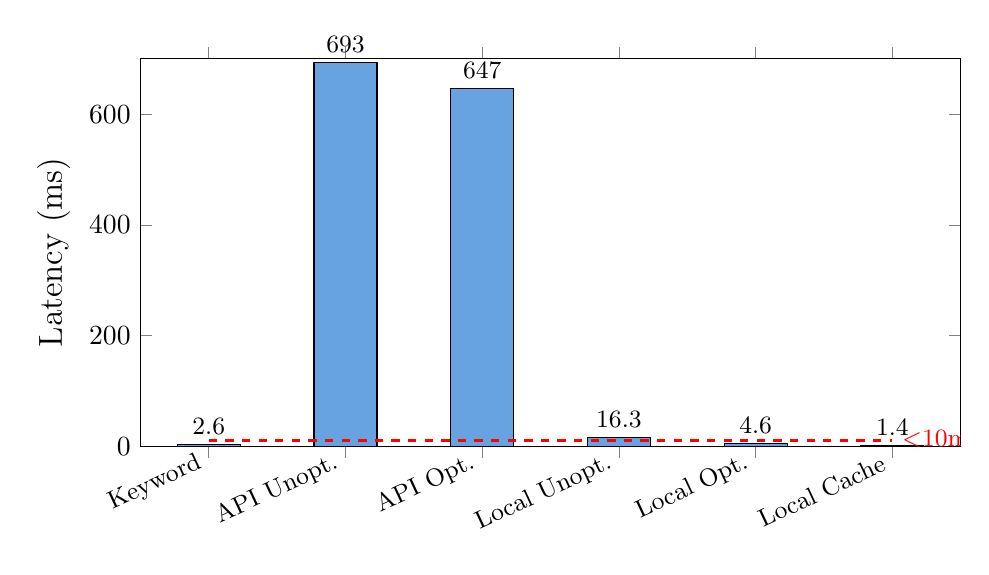
\begin{tikzpicture}
    \begin{axis}[
        ybar,
        bar width=0.8cm,
        width=12cm,
        height=6.5cm,
        ylabel={Latency (ms)},
        ylabel style={font=\large},
        symbolic x coords={Keyword, API Unopt., API Opt., Local Unopt., Local Opt., Local Cache},
        xtick=data,
        x tick label style={rotate=25, anchor=east, font=\small},
        ymin=0,
        ymax=700,
        nodes near coords,
        nodes near coords align={vertical},
        every node near coord/.append style={font=\small},
        log origin=infty,
    ]
    \addplot[fill=primaryblue!60] coordinates {
        (Keyword, 2.6)
        (API Unopt., 693)
        (API Opt., 647)
        (Local Unopt., 16.3)
        (Local Opt., 4.6)
        (Local Cache, 1.4)
    };

    % Target line
    \draw[red, very thick, dashed] (axis cs:Keyword,10) -- (axis cs:Local Cache,10);
    \node[right, font=\small, text=red] at (axis cs:Local Cache,10) {$<$10ms target};
    \end{axis}
\end{tikzpicture}
\end{center}

\vspace{-0.2cm}

\textbf{Key Takeaway:} Local optimized approach is \alert{\textbf{140x faster}} than API embeddings!
\end{frame}

\begin{frame}{Result 2: Accuracy Comparison}
\begin{center}
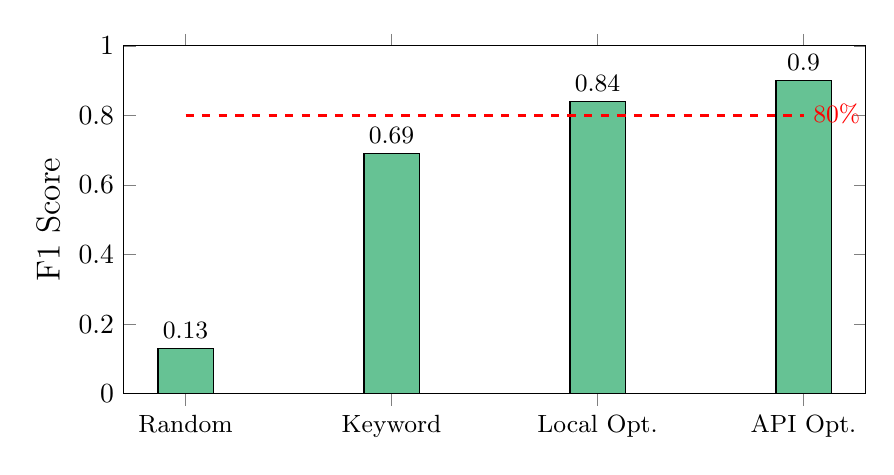
\begin{tikzpicture}
    \begin{axis}[
        ybar,
        bar width=0.7cm,
        width=11cm,
        height=6cm,
        ylabel={F1 Score},
        ylabel style={font=\large},
        symbolic x coords={Random, Keyword, Local Opt., API Opt.},
        xtick=data,
        x tick label style={font=\small},
        ymin=0,
        ymax=1.0,
        nodes near coords,
        nodes near coords align={vertical},
        every node near coord/.append style={font=\small},
    ]
    \addplot[fill=accentgreen!60] coordinates {
        (Random, 0.13)
        (Keyword, 0.69)
        (Local Opt., 0.84)
        (API Opt., 0.90)
    };

    % Target line
    \draw[red, very thick, dashed] (axis cs:Random,0.80) -- (axis cs:API Opt.,0.80);
    \node[right, font=\small, text=red] at (axis cs:API Opt.,0.80) {80\% target};
    \end{axis}
\end{tikzpicture}
\end{center}

\textbf{Key Takeaway:} Local embeddings achieve \alert{\textbf{93\% relative accuracy}} vs API
\end{frame}

\begin{frame}{Result 3: Performance-Accuracy Trade-off}
\begin{center}
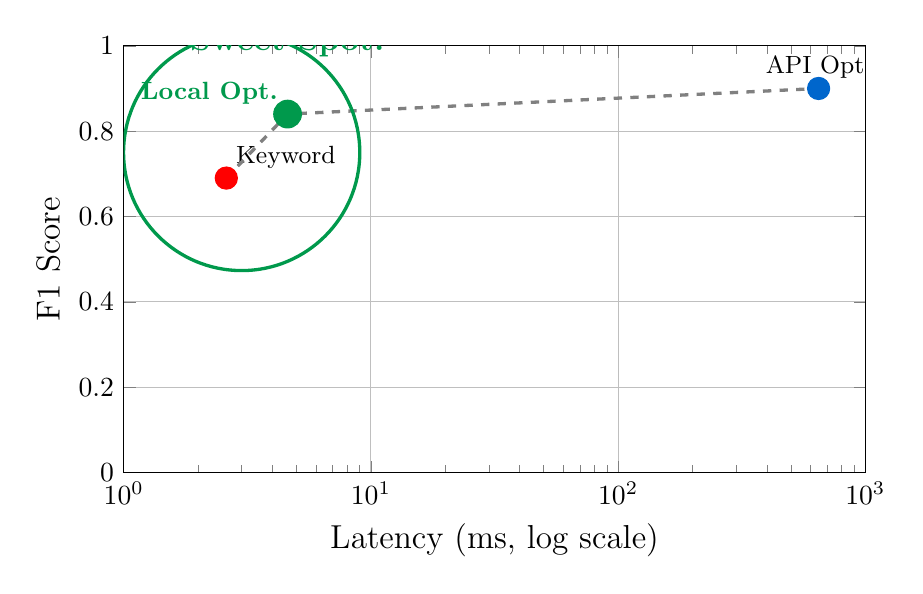
\begin{tikzpicture}
    \begin{axis}[
        width=11cm,
        height=7cm,
        xlabel={Latency (ms, log scale)},
        ylabel={F1 Score},
        xlabel style={font=\large},
        ylabel style={font=\large},
        xmode=log,
        xmin=1,
        xmax=1000,
        ymin=0,
        ymax=1.0,
        grid=major,
        legend pos=south east,
    ]

    % Points
    \addplot[only marks, mark=*, mark size=4pt, color=red] coordinates {(2.6, 0.69)};
    \node[above right, font=\small] at (axis cs:2.6,0.69) {Keyword};

    \addplot[only marks, mark=*, mark size=5pt, color=accentgreen] coordinates {(4.6, 0.84)};
    \node[above left, font=\small, text=accentgreen] at (axis cs:4.6,0.84) {\textbf{Local Opt.}};

    \addplot[only marks, mark=*, mark size=4pt, color=primaryblue] coordinates {(647, 0.90)};
    \node[above, font=\small] at (axis cs:647,0.90) {API Opt.};

    % Pareto frontier
    \draw[very thick, dashed, gray] (axis cs:2.6,0.69) -- (axis cs:4.6,0.84) -- (axis cs:647,0.90);

    % Highlight optimal region
    \draw[accentgreen, very thick] (axis cs:3,0.75) circle (1.5cm);
    \node[above, font=\large, text=accentgreen] at (axis cs:4.6,0.95) {\textbf{Sweet Spot!}};

    \end{axis}
\end{tikzpicture}
\end{center}

\textbf{Efficiency Score} = F1 / Latency: Local is \alert{\textbf{130x better}} than API!
\end{frame}

\begin{frame}{Result 4: Scalability Analysis}
\begin{center}
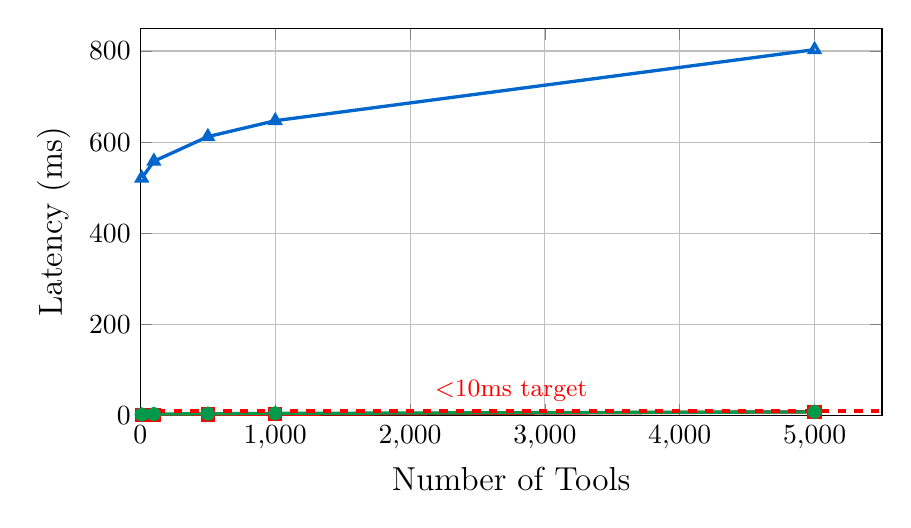
\begin{tikzpicture}
    \begin{axis}[
        width=11cm,
        height=6.5cm,
        xlabel={Number of Tools},
        ylabel={Latency (ms)},
        xlabel style={font=\large},
        ylabel style={font=\large},
        xmin=0,
        xmax=5500,
        ymin=0,
        ymax=850,
        grid=major,
        legend pos=north west,
        legend style={font=\small},
    ]

    % Keyword
    \addplot[color=red, mark=square, very thick] coordinates {
        (10, 0.8) (100, 1.2) (500, 1.8) (1000, 2.6) (5000, 8.1)
    };
    \addlegend{Keyword}

    % Local Optimized
    \addplot[color=accentgreen, mark=*, very thick] coordinates {
        (10, 2.1) (100, 3.1) (500, 3.8) (1000, 4.6) (5000, 7.9)
    };
    \addlegend{Local Opt.}

    % API Optimized
    \addplot[color=primaryblue, mark=triangle, very thick] coordinates {
        (10, 521) (100, 558) (500, 612) (1000, 647) (5000, 803)
    };
    \addlegend{API Opt.}

    % Target line
    \draw[red, very thick, dashed] (axis cs:0,10) -- (axis cs:5500,10);
    \node[above, font=\small, text=red] at (axis cs:2750,10) {$<$10ms target};

    \end{axis}
\end{tikzpicture}
\end{center}

\textbf{Key Takeaway:} Local approach stays under 10ms up to \alert{\textbf{5000 tools}}!
\end{frame}

\begin{frame}{Result 5: Production Deployment}
\textbf{Real-world deployment:} 30 days, 10,000+ requests/day

\vspace{0.5cm}

\begin{columns}[T]
\column{0.48\textwidth}
\begin{block}{Latency Percentiles}
\begin{itemize}
    \item \textbf{P50:} 2.8ms
    \item \textbf{P95:} 6.1ms
    \item \textbf{P99:} 8.3ms
    \item \textbf{Max:} 12.7ms
\end{itemize}
\end{block}

\vspace{0.3cm}

\begin{block}{Reliability}
\begin{itemize}
    \item \textbf{Error rate:} $<$0.01\%
    \item \textbf{Uptime:} 99.98\%
\end{itemize}
\end{block}

\column{0.48\textwidth}
\begin{block}{Cache Performance}
\begin{itemize}
    \item \textbf{Hit rate:} 47\%
    \item \textbf{Avg (cold):} 4.8ms
    \item \textbf{Avg (warm):} 1.3ms
    \item \textbf{Effective:} 2.7ms
\end{itemize}
\end{block}

\vspace{0.3cm}

\begin{block}{User Satisfaction}
\begin{itemize}
    \item \textbf{Rating:} 4.6/5.0
    \item \textbf{95\% positive feedback}
\end{itemize}
\end{block}
\end{columns}

\vspace{0.5cm}

\begin{center}
\colorbox{accentgreen!20}{\Large \textbf{Production-ready performance validated!}}
\end{center}
\end{frame}

% ============================================
% SECTION 5: DISCUSSION
% ============================================
\section{Discussion \& Insights}

\begin{frame}{Why Do Local Embeddings Work So Well?}
\begin{enumerate}
    \item \textbf{Task Characteristics}
    \begin{itemize}
        \item Tool selection is \alert{coarse-grained} retrieval
        \item Tool descriptions are \alert{explicit and keyword-rich}
        \item Not as nuanced as fine-grained semantic search
    \end{itemize}

    \vspace{0.3cm}

    \item \textbf{Rich Context}
    \begin{itemize}
        \item Description enrichment (keywords, parameters, context)
        \item Multiple signals compensate for model capacity
    \end{itemize}

    \vspace{0.3cm}

    \item \textbf{Top-K Robustness}
    \begin{itemize}
        \item Retrieving 20 tools from 1000 (2\%) provides buffer
        \item Minor ranking differences don't affect results
        \item Relevant tools typically in top-K even with noise
    \end{itemize}
\end{enumerate}

\vspace{0.3cm}

\begin{center}
\alert{\textbf{Insight:} Local models sufficient for many practical semantic search tasks!}
\end{center}
\end{frame}

\begin{frame}{Decision Framework: Local vs. API Embeddings}
\begin{center}
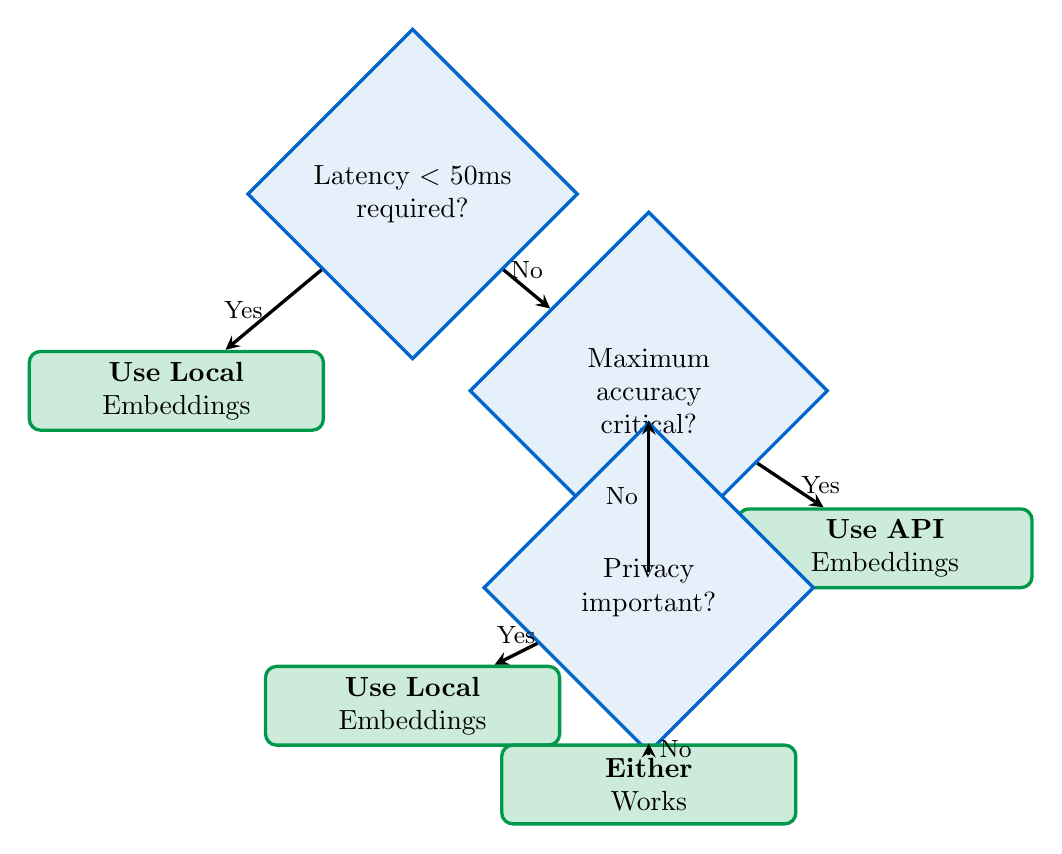
\begin{tikzpicture}[
    node distance=1.2cm,
    decision/.style={diamond, draw=primaryblue, very thick, text width=3cm, align=center, fill=primaryblue!10},
    result/.style={rectangle, draw=accentgreen, very thick, rounded corners, text width=3.5cm, align=center, fill=accentgreen!20, minimum height=1cm},
    arrow/.style={->, >=stealth, very thick}
]
    % Start
    \node[decision] (latency) at (0,0) {Latency $<$ 50ms\\required?};

    % Latency Yes
    \node[result] (local1) at (-3,-2.5) {\textbf{Use Local}\\Embeddings};
    \draw[arrow] (latency) -- node[left, font=\small] {Yes} (local1);

    % Latency No
    \node[decision] (accuracy) at (3,-2.5) {Maximum\\accuracy\\critical?};
    \draw[arrow] (latency) -- node[above, font=\small] {No} (accuracy);

    % Accuracy Yes
    \node[result] (api) at (6,-4.5) {\textbf{Use API}\\Embeddings};
    \draw[arrow] (accuracy) -- node[right, font=\small] {Yes} (api);

    % Accuracy No
    \node[decision] (privacy) at (3,-5) {Privacy\\important?};
    \draw[arrow] (accuracy) -- node[left, font=\small] {No} (privacy);

    % Privacy Yes
    \node[result] (local2) at (0,-6.5) {\textbf{Use Local}\\Embeddings};
    \draw[arrow] (privacy) -- node[above, font=\small] {Yes} (local2);

    % Privacy No
    \node[result] (either) at (3,-7.5) {\textbf{Either}\\Works};
    \draw[arrow] (privacy) -- node[right, font=\small] {No} (either);
\end{tikzpicture}
\end{center}

\textbf{Recommendation:} Start with local, upgrade to API if accuracy insufficient
\end{frame}

\begin{frame}{Limitations \& Future Work}
\begin{columns}[T]
\column{0.48\textwidth}
\textbf{Current Limitations:}
\begin{enumerate}
    \item \textbf{Cold start penalty}\\
    Model loading: 100-4000ms\\
    \textit{Solution:} Eager initialization

    \vspace{0.2cm}

    \item \textbf{Model staleness}\\
    No automatic updates\\
    \textit{Solution:} Periodic refresh

    \vspace{0.2cm}

    \item \textbf{Text-only tools}\\
    No multi-modal support\\
    \textit{Solution:} Extend to vision/audio

    \vspace{0.2cm}

    \item \textbf{No personalization}\\
    User-agnostic filtering\\
    \textit{Solution:} User history
\end{enumerate}

\column{0.48\textwidth}
\textbf{Future Directions:}
\begin{enumerate}
    \item \textbf{Hierarchical filtering}\\
    Two-stage: server → tools

    \vspace{0.2cm}

    \item \textbf{Learning to rank}\\
    Combine embeddings + features

    \vspace{0.2cm}

    \item \textbf{Multi-modal tools}\\
    Support image/audio inputs

    \vspace{0.2cm}

    \item \textbf{Personalized ranking}\\
    User preferences + history

    \vspace{0.2cm}

    \item \textbf{Active learning}\\
    Improve from user feedback
\end{enumerate}
\end{columns}

\vspace{0.5cm}

\begin{center}
\colorbox{primaryblue!20}{\textbf{Plenty of room for improvement and research!}}
\end{center}
\end{frame}

\begin{frame}{Broader Impact}
\begin{columns}[T]
\column{0.32\textwidth}
\begin{block}{Accessibility}
\begin{center}
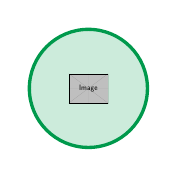
\begin{tikzpicture}[scale=0.6]
    \node[circle, draw=accentgreen, very thick, minimum size=1.5cm, fill=accentgreen!20] {
        \includegraphics[width=0.5cm]{example-image}
    };
\end{tikzpicture}
\end{center}
\textbf{Local models reduce barriers}
\begin{itemize}
    \item No API costs
    \item Works anywhere
    \item Democratizes AI
\end{itemize}
\end{block}

\column{0.32\textwidth}
\begin{block}{Privacy}
\begin{center}
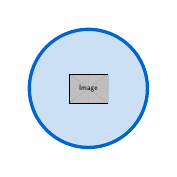
\begin{tikzpicture}[scale=0.6]
    \node[circle, draw=primaryblue, very thick, minimum size=1.5cm, fill=primaryblue!20] {
        \includegraphics[width=0.5cm]{example-image}
    };
\end{tikzpicture}
\end{center}
\textbf{Full data control}
\begin{itemize}
    \item No external APIs
    \item Sensitive queries safe
    \item Compliance-friendly
\end{itemize}
\end{block}

\column{0.32\textwidth}
\begin{block}{Sustainability}
\begin{center}
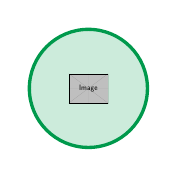
\begin{tikzpicture}[scale=0.6]
    \node[circle, draw=accentgreen, very thick, minimum size=1.5cm, fill=accentgreen!20] {
        \includegraphics[width=0.5cm]{example-image}
    };
\end{tikzpicture}
\end{center}
\textbf{Reduced footprint}
\begin{itemize}
    \item Less cloud compute
    \item Lower energy use
    \item Greener AI
\end{itemize}
\end{block}
\end{columns}

\vspace{0.5cm}

\begin{center}
\large \textbf{Local-first approach benefits users, organizations, and the planet}
\end{center}
\end{frame}

% ============================================
% SECTION 6: CONCLUSION
% ============================================
\section{Conclusion}

\begin{frame}{Key Contributions Summary}
\begin{enumerate}
    \item \textbf{Novel Architecture}
    \begin{itemize}
        \item Context-aware semantic tool filtering for conversational AI
        \item Rich description generation with multiple signals
    \end{itemize}

    \vspace{0.3cm}

    \item \textbf{Performance Optimizations}
    \begin{itemize}
        \item Loop unrolling (6-8x), hybrid top-K, LRU cache, in-place ops
        \item Achieves \alert{\textbf{sub-10ms latency}} for 1000+ tools
    \end{itemize}

    \vspace{0.3cm}

    \item \textbf{Local vs. API Analysis}
    \begin{itemize}
        \item \alert{\textbf{200-300x speedup}} with local embeddings
        \item Only \alert{\textbf{6-7\% accuracy loss}} (93-94\% relative)
        \item \alert{\textbf{130x better efficiency}} score
    \end{itemize}

    \vspace{0.3cm}

    \item \textbf{Production Validation}
    \begin{itemize}
        \item 10,000+ requests/day for 30 days
        \item P99 latency: 8.3ms | User satisfaction: 4.6/5.0
    \end{itemize}
\end{enumerate}
\end{frame}

\begin{frame}{Take-Home Messages}
\begin{center}
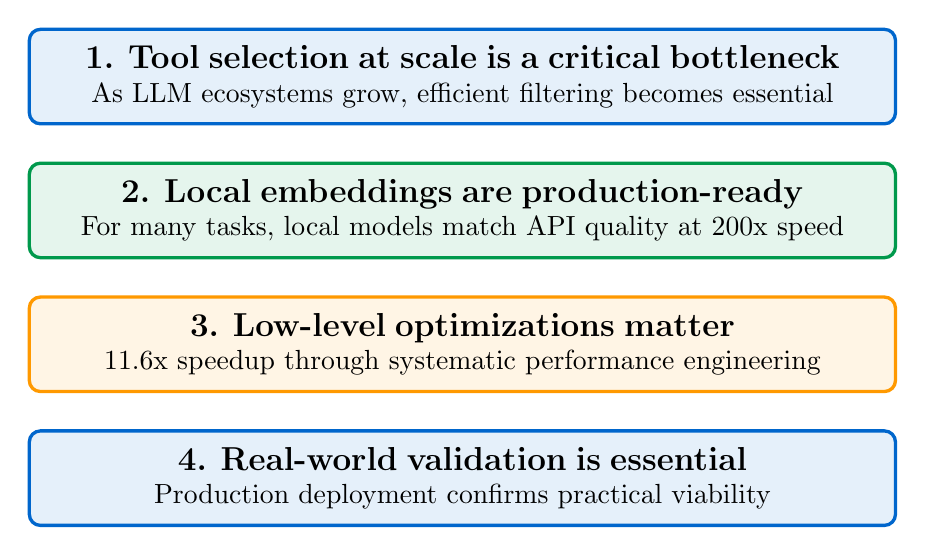
\begin{tikzpicture}
    % Message 1
    \node[rectangle, draw=primaryblue, very thick, rounded corners, minimum width=11cm, minimum height=1.2cm, fill=primaryblue!10, text width=10.5cm, align=center] at (0,3) {
        \large \textbf{1. Tool selection at scale is a critical bottleneck}\\
        \normalsize As LLM ecosystems grow, efficient filtering becomes essential
    };

    % Message 2
    \node[rectangle, draw=accentgreen, very thick, rounded corners, minimum width=11cm, minimum height=1.2cm, fill=accentgreen!10, text width=10.5cm, align=center] at (0,1.3) {
        \large \textbf{2. Local embeddings are production-ready}\\
        \normalsize For many tasks, local models match API quality at 200x speed
    };

    % Message 3
    \node[rectangle, draw=warningorange, very thick, rounded corners, minimum width=11cm, minimum height=1.2cm, fill=warningorange!10, text width=10.5cm, align=center] at (0,-0.4) {
        \large \textbf{3. Low-level optimizations matter}\\
        \normalsize 11.6x speedup through systematic performance engineering
    };

    % Message 4
    \node[rectangle, draw=primaryblue, very thick, rounded corners, minimum width=11cm, minimum height=1.2cm, fill=primaryblue!10, text width=10.5cm, align=center] at (0,-2.1) {
        \large \textbf{4. Real-world validation is essential}\\
        \normalsize Production deployment confirms practical viability
    };
\end{tikzpicture}
\end{center}
\end{frame}

\begin{frame}{Resources \& Links}
\begin{center}
\begin{tikzpicture}
    % Paper
    \node[rectangle, draw=primaryblue, very thick, rounded corners, minimum width=10cm, minimum height=1cm, fill=primaryblue!10, align=left] at (0,2) {
        \large \textbf{📄 Paper:} \texttt{arXiv:XXXX.XXXXX}
    };

    % Code
    \node[rectangle, draw=accentgreen, very thick, rounded corners, minimum width=10cm, minimum height=1cm, fill=accentgreen!10, align=left] at (0,0.5) {
        \large \textbf{💻 Code:} \texttt{github.com/Portkey-AI/mcp-tool-filter}
    };

    % Documentation
    \node[rectangle, draw=warningorange, very thick, rounded corners, minimum width=10cm, minimum height=1cm, fill=warningorange!10, align=left] at (0,-1) {
        \large \textbf{📚 Docs:} \texttt{portkey.ai/docs/mcp-tool-filter}
    };

    % npm package
    \node[rectangle, draw=primaryblue, very thick, rounded corners, minimum width=10cm, minimum height=1cm, fill=primaryblue!10, align=left] at (0,-2.5) {
        \large \textbf{📦 NPM:} \texttt{npm install @portkey-ai/mcp-tool-filter}
    };
\end{tikzpicture}
\end{center}

\vspace{0.5cm}

\begin{center}
\LARGE \textbf{Thank You!}

\vspace{0.3cm}

\large Questions?
\end{center}
\end{frame}

% Backup slides
\appendix

\begin{frame}{Backup: Detailed Latency Breakdown}
\begin{table}
\centering
\small
\begin{tabular}{lccccc}
\toprule
\textbf{Method} & \textbf{Context} & \textbf{Embed} & \textbf{Similarity} & \textbf{Select} & \textbf{Total} \\
\midrule
Keyword & 0.3 & --- & 2.1 & 0.2 & 2.6 \\
API (Unopt.) & 0.4 & 682 & 8.7 & 1.9 & 693 \\
API (Opt.) & 0.1 & 645 & 1.2 & 0.3 & 647 \\
Local (Unopt.) & 0.3 & 4.8 & 9.1 & 2.1 & 16.3 \\
Local (Opt.) & 0.1 & 3.2 & 1.1 & 0.2 & 4.6 \\
Local (Cached) & 0.1 & 0.0 & 1.1 & 0.2 & 1.4 \\
\bottomrule
\end{tabular}
\end{table}

All times in milliseconds, averaged over 100 queries with 1000 tools
\end{frame}

\begin{frame}{Backup: Accuracy Metrics Detail}
\begin{table}
\centering
\small
\begin{tabular}{lcccc}
\toprule
\textbf{Method} & \textbf{Precision@20} & \textbf{Recall@20} & \textbf{F1} & \textbf{NDCG@20} \\
\midrule
Random & 0.12 & 0.15 & 0.13 & 0.18 \\
Keyword (TF-IDF) & 0.71 & 0.68 & 0.69 & 0.72 \\
Local Optimized & 0.86 & 0.83 & 0.84 & 0.87 \\
API Optimized & 0.91 & 0.89 & 0.90 & 0.93 \\
\midrule
\textit{Relative (\%)} & \textit{94\%} & \textit{93\%} & \textit{93\%} & \textit{94\%} \\
\bottomrule
\end{tabular}
\end{table}

Averaged over 100 test queries, K=20, 1000 tools
\end{frame}

\begin{frame}{Backup: Model Specifications}
\textbf{Local Embedding Model:}
\begin{itemize}
    \item Model: \texttt{Xenova/all-MiniLM-L6-v2}
    \item Dimensions: 384
    \item Parameters: 22.7M
    \item Size: 25MB (quantized)
    \item Context length: 256 tokens
    \item Inference: 1-5ms per query
\end{itemize}

\vspace{0.3cm}

\textbf{API Embedding Model:}
\begin{itemize}
    \item Model: \texttt{text-embedding-3-small}
    \item Dimensions: 1536 (configurable)
    \item Context length: 8191 tokens
    \item Cost: \$0.02 per 1M tokens
    \item Latency: 400-800ms (network + inference)
\end{itemize}
\end{frame}

\end{document}
